\anonsection{Задание 8}
\anonsubsection{Формулировка задания}

Применить метод Монте--Карло к решению первой краевой задачи для двумерного 
 уравнения Лапласа в единичном круге:
\begin{equation} \label{Dirichlet}
\left\lbrace
\begin{array}{lcr}
\Delta u=0,(x,y)\in D,\\
u|_{\delta D}=f(x,y),\\
u\in C^2(D),f\in C(\delta D),\\
D=\lbrace x,y:x^2+y^2\leqslant1\rbrace.
\end{array}
\right.
\end{equation}

Для функции \( f(x,y)=x^2-y^2 \) найти аналитическое решение и сравнить с 
 полученным по методу Монте--Карло.



\anonsubsection{Алгоритм решения}
Для приближенного решения задачи выберем на плоскости достаточно мелкую
квадратную сетку с шагом $h$. В таком случае, координатами узлов сетки 
 можно считать $x_j = jh, \ y_l = lh.$

\begin{definition}
	Будем называть узел сетки $(j, l)$ внутренним, если он и все четыре 
     соседних с ним узла
	$(j-1, l), \ (j + 1, l), \ (j, l - 1), \ (j, l + 1)$ принадлежат $D + 
     \delta D$, в противном случае узел $(j, l)$, принадлежащий $D + 
     \delta D$, будем называть граничным.
\end{definition} 

Во внутреннем узле \( (x_i,y_j) \) уравнение Лапласа \( u_{xx}+u_{yy}=0 \) 
 заменим разностным уравнением
\[
 \dfrac{u_{i + 1, j} - 2 u_{i, j} + u_{i - 1, j}}{h^2} + \dfrac{u_{i, j + 1} - 
  2 u_{i, j} + u_{i, j - 1}} {h^2} = 0,
\]
которое можно переписать в виде
\begin{equation} \label{internal}
u_{i,j}=\dfrac{1}{4}(u_{i-1,j}+u_{i+1,j}+u_{i,j-1}+u_{i,j+1}).
\end{equation}

В граничном узле положим
\begin{equation} \label{borders}
u_{i,j}=f_{i,j}.
\end{equation}

 

Представим себе частицу \( M \), которая совершает равномерное случайное 
 блуждание по узлам сетки. А именно, находясь во внутреннем узле 
 \( (x_i,y_j) \) сетки, эта частица за один переход с одинаковой 
 вероятностью \( 1/4 \) может переместиться в один из четырёх соседних 
 узлов, причём каждый такой единичный переход случаен и не зависит от 
 положения частицы и истории её передвижений. Будем считать, что блуждание 
 заканчивается, как только частица попадает в граничный узел. 

Пусть \( P(i,j,p,q) \)~---~вероятность того, что траектория частицы, 
 вышедшей из узла \( (x_i,y_j) \), закончится в граничном узле 
 \( (x_q,y_q) \). Так как блуждение точки неизбежно заканчивается на 
 границе в первой же точке выхода её на границу, то
\[
 \sum\limits_{(x_p,y_q)\in\delta D_h}P(i,j,p,q)=1,
\]
причём если \( (p',q'), (p,q)\in\delta D_h \), то
\[
P(p',q',p,q)=\begin{cases}
1,&(p'-p)^2+(q'-q)^2=0,\\
0,&(p'-p)^2+(q'-q)^2\ne0.
\end{cases}
\]

Составим сумму
\[
 v_{i,j}=\sum\limits_{(x_p,y_q)\in\delta D_h}P(i,j,p,q)f_{pq}.
\]

Если рассматривать функцию \( f(x,y) \) как случайную величину, принимающую 
 значения \( f_{pq} \) на границе \( \delta D_h \), то написанная выше 
 сумма представляет собой математическое ожидание функции \( f(x,y) \) на 
 границе \( \delta D_h \) для траекторий, начинающихся в узле \( (x_i,y_j) \). 
 Тогда в силу закона больших чисел можно аппроксимировать математическое 
 ожидание выборочным средним:
\[
 v_{i, j} \approx \dfrac{1}{N} \sum\limits_{k = 1}^{N} f \left( x_p^{(k)}, 
 y_q^{(k)} \right).
\]

Частица, начавшая своё случайное блуждание из внутреннего узла 
 \( (x_i,y_j) \), после первого шага с вероятностью, равной \( 1/4 \), 
 попадает в один из соседних четырёх узлов. Откуда по формуле полной 
 вероятности
\[
 v_{i, j} = \dfrac{1}{4} \sum\limits_{(x_p,y_q) \in\delta D_h} 
 (P(i - 1, j, p, q) + P(i + 1, j, p, q) + P(i, j - 1, p, q) + 
 P(i, j + 2, p, q))f_{p q} =
\]
\[
 = \dfrac{1}{4}(v_{i - 1, j} + v_{i + 1, j} + v_{i, j - 1} + v_{i,j + 1}).
\]
То есть во внутреннем узле \( (x_i, y_j) \)
\begin{equation} \label{internal_new}
    v_{i, j} = \dfrac{1}{4}(v_{i - 1, j} + v_{i + 1, j} + v_{i, j - 1} + 
     v_{i, j + 1}),
\end{equation}
в граничном узле
\begin{equation} \label{borders_new}
    v_{i, j} = f_{i, j}.
\end{equation}
 

По теореме о существовании решения внутренней задачи Дирихле решение 
 задачи ~ (\ref{Dirichlet}) существует. Найдем его для конкретной функции 
 \( f(x,y)=x^2-y^2 \). Будем искать его в виде \( u(x,y)=Ax^2+By^2+C \). 
 Подставив его в формулировку задачи, получим следующие условия на 
 коэффициенты:
\[
 \left\lbrace
 \begin{array}{rcl}
    A + B & = & 0,\\
    A - B & = & 2,\\
    B + C & = & -1;
\end{array}
\right.\quad\Longleftrightarrow\quad
\left\lbrace
\begin{array}{rcl}
A&=&1,\\
B&=&-1,\\
C&=&0;
\end{array}
\right.
\]

То есть мы получили, что функция \( u(x,y)=x^2-y^2 \) является решением 
 задачи~(\ref{Dirichlet}), причём решение единственно.

Согласно приведённым выше выкладкам, численное решение может быть найдено 
 по следующему алгоритму:

\begin{enumerate}
	\item Построим квадратную сетку на \( [-1,1]\times[-1,1] \) с шагом 
     \( \Delta \).
	
	\item Функцию во всех узлах, не принадлежащих кругу, положим равной 
     None.
	
	\item Все точки круга разделим на граничные и внутренние:
	
	\begin{itemize}
		\item В граничных точках положим \( u(x,y)=f(x,y) \).
		
		\item Значение в каждой внутренней точке получим следующим образом. 
         Попав во внутреннюю точку \( (x_i,y_j) \), проведём серию из 
         \( n \) случайных блужданий. Тогда
		\[
		u(x_i,y_j) = \dfrac{1}{n} \sum\limits_{k = 1}^{n} f \left( x_i^{(k)}, 
         y_i^{(k)} \right), 
		\]
		где \( \left( x_i^{(k)}, y_i^{(k)} \right) \)~---~граничная точка, в 
         которой завершилось \( k \)-е блуждание.
	\end{itemize}
\end{enumerate}

На Рис.\eqref{fig:boundary_solutions} изображены графики решения полученного по методу Монте-Карло
 и аналитического решения.

\begin{figure}[ht]
    \centering
    \begin{subfigure}[b]{0.45\textwidth}
        \centering
        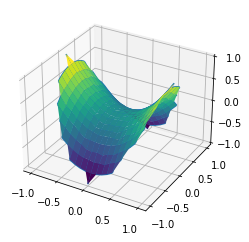
\includegraphics[width=\textwidth]{./resources/boundary_problem_emp.png}
        \caption{Решение по методу Монте-Карло.}
        \label{subfig:boundary_emp}
    \end{subfigure}
    \hfill
    \begin{subfigure}[b]{0.45\textwidth}
        \centering
        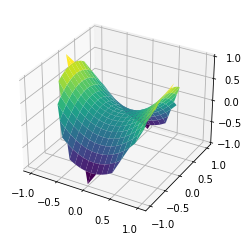
\includegraphics[width=\textwidth]{./resources/boundary_problem_an.png}
        \caption{Аналитическое решение: $ x^2 - y^2. $}
        \label{subfig:boundary_an}
    \end{subfigure}
    \caption{Решения задачи Дирихле.}
    \label{fig:boundary_solutions}
\end{figure}